\documentclass{article}
\usepackage[utf8]{inputenc}
\usepackage[T2A]{fontenc}
\usepackage{xcolor}
\usepackage[english,russian]
{babel}
\usepackage{amsfonts}
\usepackage{listings}
\usepackage{graphicx}

\definecolor{codegreen}{rgb}{0,0.6,0}
\definecolor{codegray}{rgb}{0.5,0.5,0.5}
\definecolor{codepurple}{rgb}{0.58,0,0.82}
\definecolor{backcolour}{rgb}{0.95,0.95,0.92}

\lstdefinestyle{mystyle}{
    backgroundcolor=\color{backcolour},   
    commentstyle=\color{codegreen},
    keywordstyle=\color{magenta},
    numberstyle=\tiny\color{codegray},
    stringstyle=\color{codepurple},
    basicstyle=\ttfamily\footnotesize,
    breakatwhitespace=false,         
    breaklines=true,
    captionpos=b,                    
    keepspaces=true,                 
    numbers=left,                    
    numbersep=5pt,                  
    showspaces=false,                
    showstringspaces=false,
    showtabs=false,                  
    tabsize=2
}
\lstset{style=mystyle, language=[Auto]Lisp, inputencoding=cp1251}

\begin{document}
\Large\textbf{Лабораторная работа №1}

\textbf{Выполнил: Кузнецов Павел М3207}

\textcolor{blue}{\textit{осваиваю \LaTeX:)}}
\vspace{5mm}

\textbf{Задача 1.} Пусть выборка $X_1,\; \ldots\;, X_n$ соответсвует классу распределений $F_\theta,\,\theta\in E\subset \mathbb{R}$. При каком минимальном объёме выборки $n$ равномерно для $\theta \in E$ выборочное среднее отличается от математического ожидания $\mu_\theta$ не более чем на $\varepsilon>0$ с вероятностью, не меньшей $1 - \delta,\,\delta \in (0,1)$ ? Сгенерировать $500$ выборок найденного объема при $\varepsilon=0.01$ и $\delta=0.05$ из указанного распределения $F_\theta$ при конкретном параметре $\theta$ и посчитать, сколько раз выборочное среднее отличается от математического ожидания $\mu_\theta$ более чем на $\varepsilon$.\\$F_\theta = Bern(p),\,p \in (0,1),\,p=2/3$
\vspace{5mm}

\textbf{Решение:}

    sum-up: у нас есть некоторая выборка $X_1,\; \ldots\;, X_n$, 
    которая соответсвует классу распределений $F_\theta = Bern(p),\\p \in (0,1)$, нужно найти min $n : P(|\bar X_n - \mu| \leq \varepsilon) \geq 1 - \delta$
\begin {center}
$P(|\bar X_n - \mu| \leq \varepsilon) = P(\frac{\sqrt{n}|\bar X_n - \mu|}{\sigma} \leq \frac{\sqrt{n}\varepsilon}{\sigma}) \approx 2\Phi(\frac{\sqrt{n}\varepsilon}{\sigma})$ (из центральной предельной теоремы, плотность ст. нормального распределения симметрична)

$2\Phi(\frac{\sqrt{n}\varepsilon}{\sigma}) \geq 1 - \delta$

$\Phi(\frac{\sqrt{n}\varepsilon}{\sigma}) \geq \frac{1 - \delta}{2}$

(так как функция Лапласа нормального распределения возрастает от аргумента, минимальное $n$ будет при минимальном значении $\Phi$)

$\Phi(\frac{\sqrt{n}\varepsilon}{\sigma}) = \frac{1 -\delta}{2}$

$\frac{\sqrt{n}\varepsilon}{\sigma} = \Phi^{-1}(\frac{1 - \delta}{2})$
\newpage
$n_{min} = (\frac{\sigma\Phi^{-1}(\frac{1 - \delta}{2})}{\varepsilon})^2$
\end{center}
Найдём конкретные значение $n_{min}$ при заданных значениях $\theta, \varepsilon, \delta$:
\begin{lstlisting}[language=Python, mathescape=true, breaklines=true]
    import numpy
    from scipy.stats import norm
    
    #mathematical expectation
    p = 2/3

    eps = 0.01
    delta = 0.05

    #standard deviation from the Bernoulli distribution
    sigma = numpy.sqrt(p * (1 - p))
    
    n = pow(sigma*norm.ppf(1 - delta/2)/eps,2)
    n_min = round(n)
    print(n_min)
\end{lstlisting}
Получившееся значение $n_{min} = 8537$.

Сгенерируем $500$ выборок найденного объема при \\
$\varepsilon=0.01$ и $\delta=0.05$ из указанного распределения $F_p$ при конкретном параметре $p$ и посчитаем, сколько раз выборочное среднее отличается от математического ожидания $\mu_p$ более чем на $\varepsilon$:

\begin{lstlisting}[language=Python, mathescape=true, breaklines=true]
    for i in range(500):
        X = numpy.random.binomial(n, p)/n
        if (abs(X - p) > eps):
            count += 1
\end{lstlisting}
Вывод:

Выборочное среднее отличается от мат. ожидания более чем на epsilon 22 раз.
Это соответсвует 4.4 \% от 500 выборок.

\newpage
\textbf{Задача 2-4.} В файле mobile\_phones.csv приведены данные о мобильных телефонах. В сколько моделей можно вставить 2 сим-карты, сколько поддерживают 3G, каково наибольшее число ядер у процессора? Рассчитайте выборочное среднее, выборочную дисперсию, выборочную медиану и выборочную квантиль порядка 2/5, построить график эмпирической функции распределения, гистограмму и box-plot для емкости аккумулятора для всей совокупности и в отдельности для поддерживающих/не поддерживающих Wi-Fi.
\vspace{5mm}

\textbf{Решение: (код)}

\begin{lstlisting}[caption={Imports},label={lst:label},language=Python, mathescape=true, breaklines=true]
    import numpy
    from scipy.stats import norm
    import pandas
    import matplotlib.pyplot as plt
    import statsmodels.api as statsm
\end{lstlisting}

\begin{lstlisting}[language=Python, mathescape=true, breaklines=true]

    data = pandas.read_csv("/Users/frogge/proggs/mathstatLabs/lab-1/mobile_phones.csv")
    # how many models are available to install 2 sim cards
    print(data['dual_sim'].sum())

    # how many models support 3-G
    print(data['three_g'].sum())

    # maximum number of cores
    print(data['n_cores'].max())
\end{lstlisting}
Получившиеся значения:

available to install 2 sim cards = 1019

support 3-G = 1523

maximum numb of cores = 8

\newpage
Далее считаем значения (указанные в задании), строим график, гистограмму и box-plot для емкостей аккумулятора при разных выборках:
\begin{lstlisting}[caption={for all data}, label={lst:label}, language=Python, mathescape=true, breaklines=true]
new_data = data['battery_power']

# selective mean
print(round(new_data.mean(), 4))

# dispersion
print(round(new_data.var(), 4))

# median
print(round(new_data.median(), 4))

# quantile 2/5
print(round(new_data.quantile(q = 0.4), 4))

x = numpy.linspace(min(new_data), max(new_data))
y = statsm.distributions.ECDF(new_data)(x)
plt.step(x, y)
plt.title("Graph of ecdf")
plt.show()
#plt.hist(new_data, histtype='step', cumulative=True, bins=len(sample))     -     another way to plot a graph

plt.hist(new_data)
plt.title("Histogram")
plt.show()

plt.boxplot(new_data)
plt.title("Box-plot")
plt.show()
\end{lstlisting}
Получившиеся значения:

Выборочное среднее = 1238.5185

Выборочная дисперсия = 193088.3598

Выборочная медиана = 1226.0

Выборочная квантиль порядка 2/5 = 1076.0

Графики в приложении
\vspace{5mm}

Далее считаем для выборки из даты, только для моделей поддерживающих WI-FI и наоборот, код остаётся прежним меняем только значение $new\textunderscore data$
\begin{lstlisting}[language=Python, mathescape=true, breaklines=true]
    new_data = data[data['wifi'] == 1]['battery_power'] #with wf
    new_data = data[data['wifi'] == 0]['battery_power'] #without wf
\end{lstlisting}

Получившиеся значения:

Выборочное среднее with wf = 1234.9043

Выборочная дисперсия with wf= 190296.4005

Выборочная медиана with wf= 1233.0

Выборочная квантиль порядка 2/5 with wf = 1077.8

Выборочное среднее without= 1242.2353

Выборочная дисперсия without= 196128.438

Выборочная медиана without= 1222.0

Выборочная квантиль порядка 2/5 without= 1076.8
\vspace{5mm}

\newpage
\textbf{Приложение}

\begin{figure}[!h]
\begin{center}
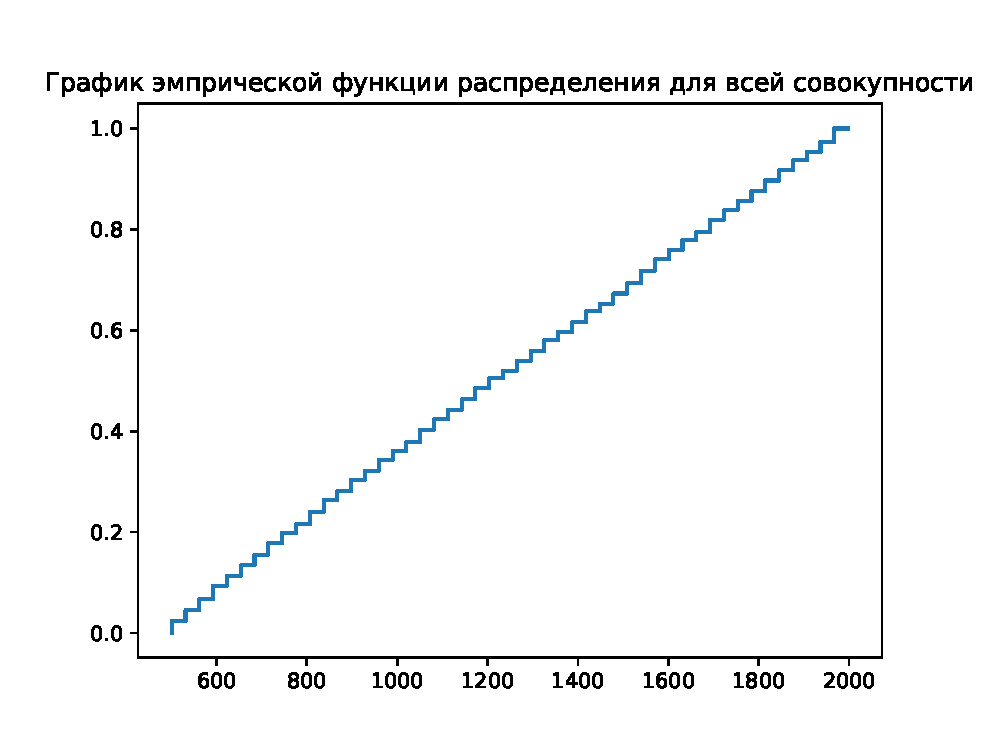
\includegraphics [scale=0.4]{images/ecdf1.eps}
\end{center}
\end{figure}

\begin{figure}[!h]
\begin{center}
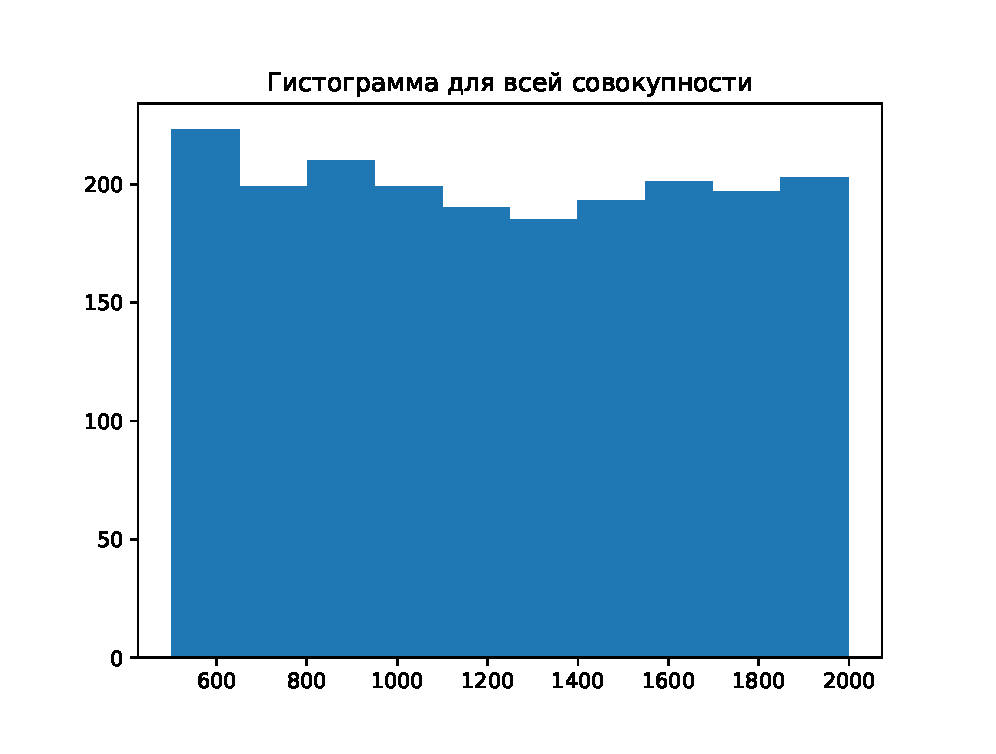
\includegraphics [scale=0.4]{images/hist1.eps}
\end{center}
\end{figure}

\begin{figure}[!h]
\begin{center}
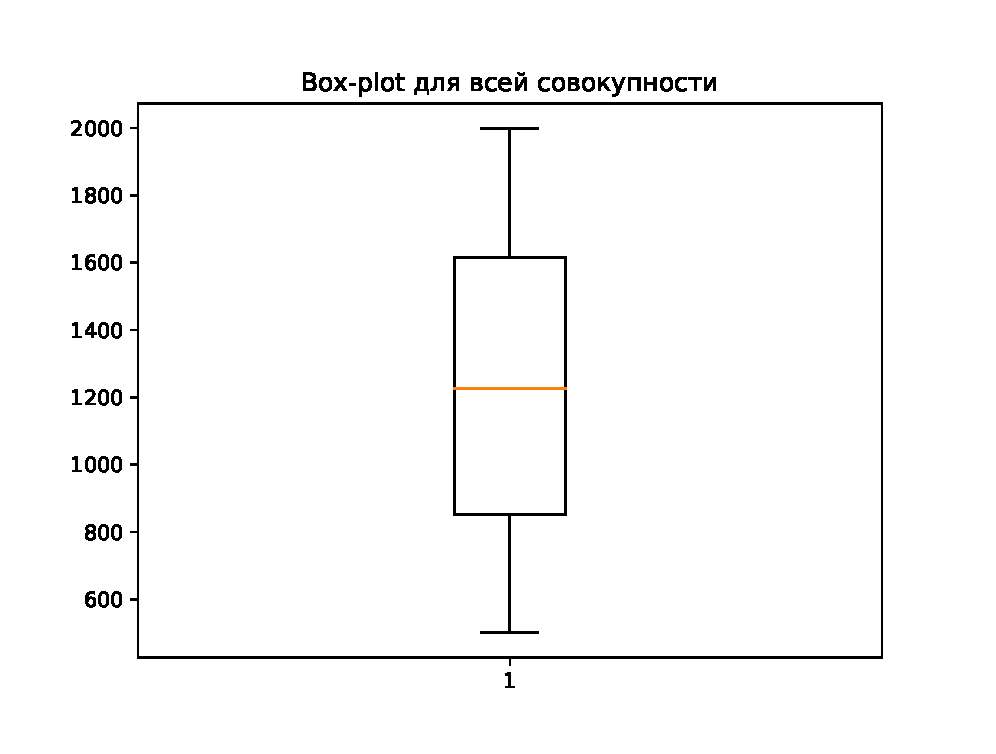
\includegraphics [scale=0.4]{images/box1.eps}
\end{center}
\end{figure}

\begin{figure}[!t]
\begin{center}
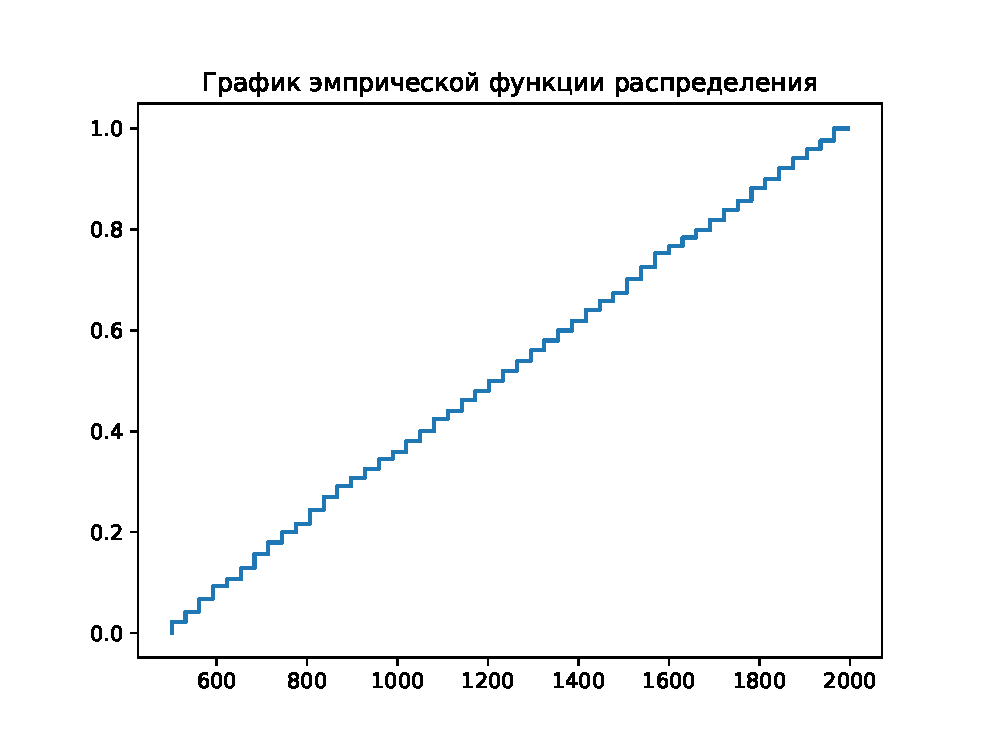
\includegraphics [scale=0.4]{images/ecdf2.eps}
\end{center}
\end{figure}

\begin{figure}[!h]
\begin{center}
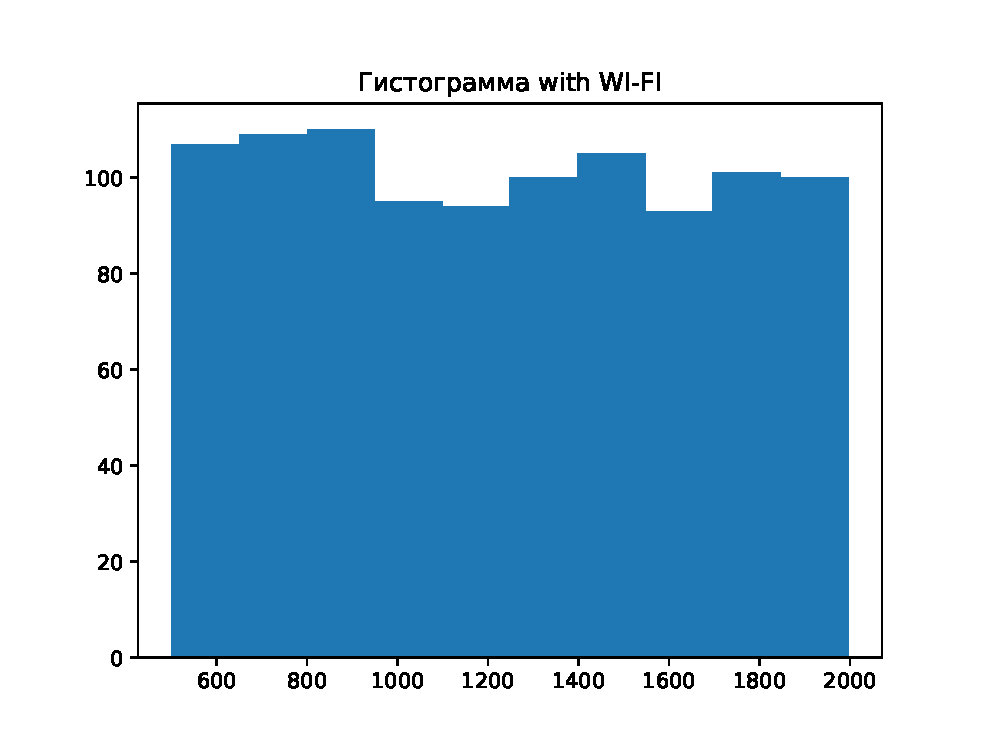
\includegraphics [scale=0.4]{images/hist2.eps}
\end{center}
\end{figure}

\begin{figure}[!h]
\begin{center}
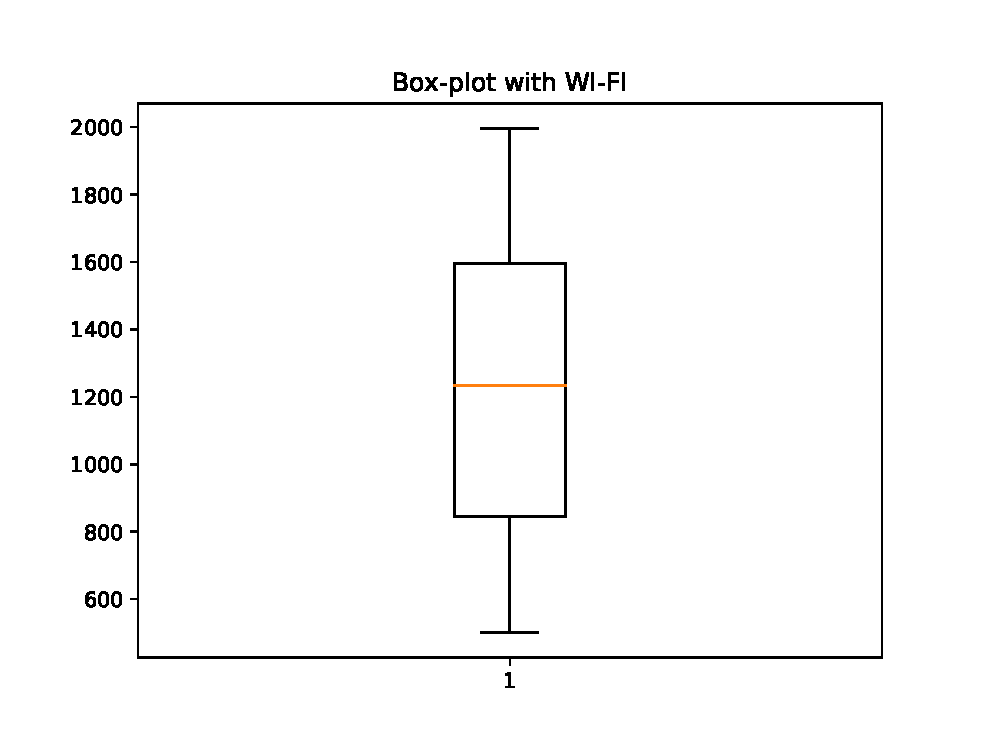
\includegraphics [scale=0.4]{images/box2.eps}
\end{center}
\end{figure}

\begin{figure}[!h]
\begin{center}
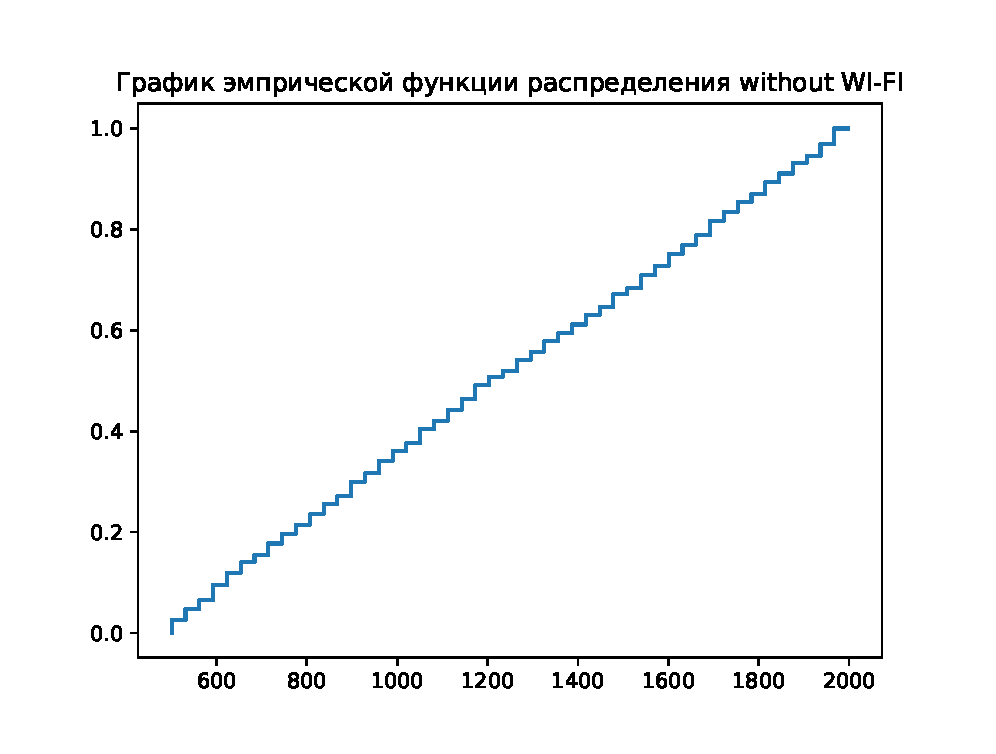
\includegraphics [scale=0.4]{images/ecdf3.eps}
\end{center}
\end{figure}

\begin{figure}[!h]
\begin{center}
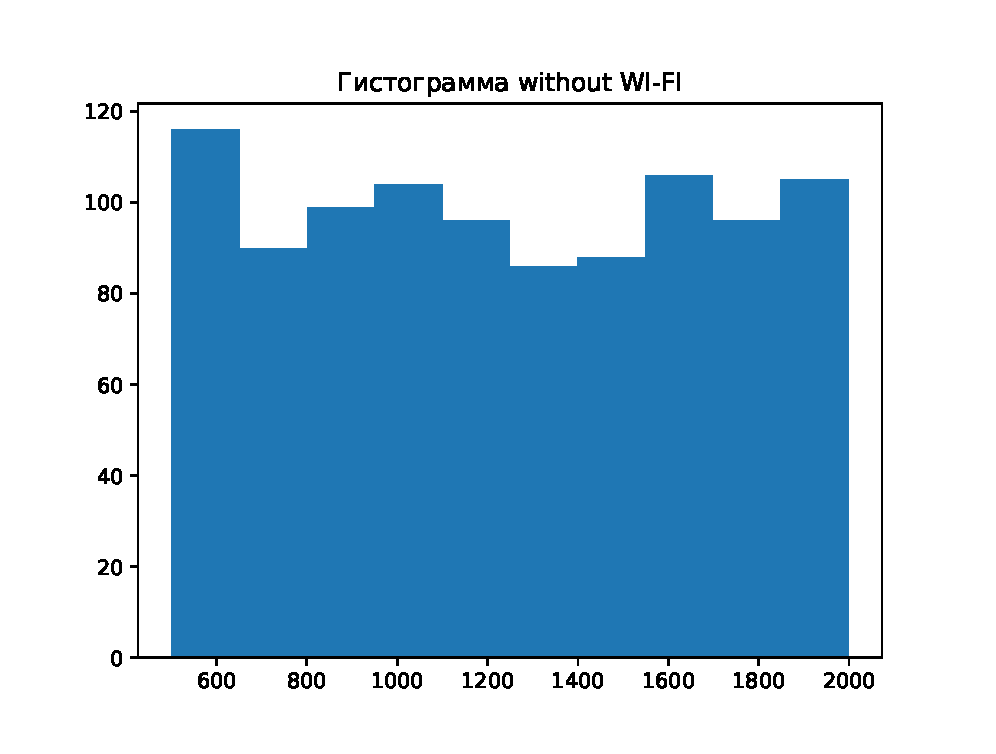
\includegraphics [scale=0.4]{images/hist3.eps}
\end{center}
\end{figure}

\begin{figure}[!h]
\begin{center}
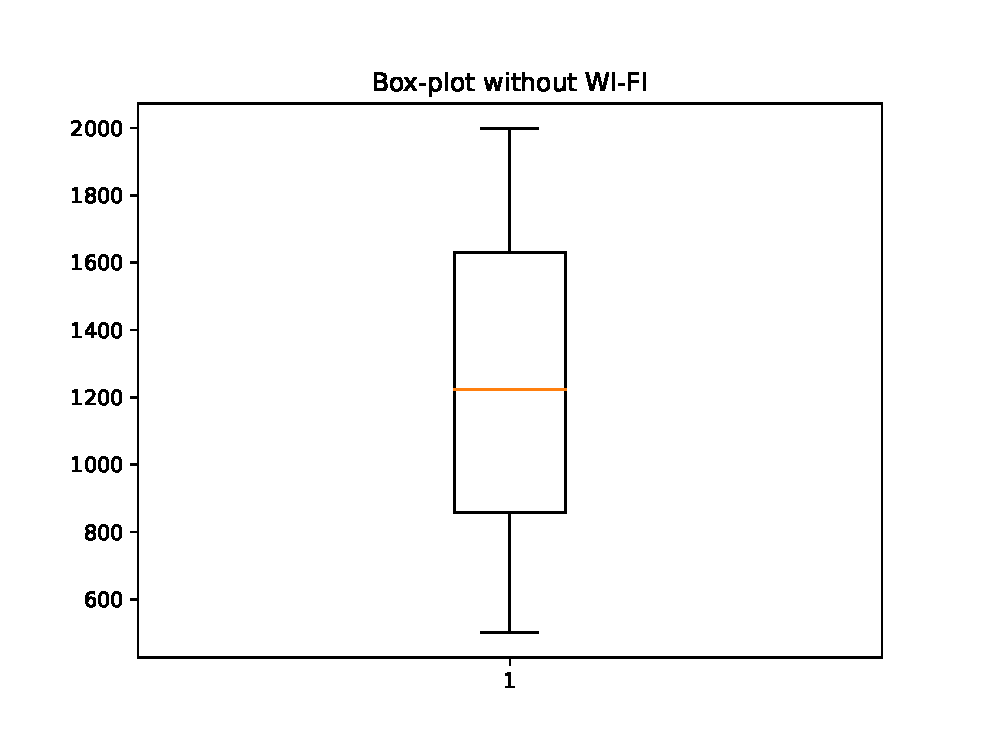
\includegraphics [scale=0.4]{images/box3.eps}
\end{center}
\end{figure}

\end{document}
